\documentclass[a4paper,11pt]{article}

\usepackage[T1]{fontenc}
\usepackage[utf8]{inputenc}
\usepackage[english]{babel}
\usepackage[top=3cm, left=2cm, textwidth=17cm, textheight=24cm]{geometry}
\usepackage{times}
\usepackage{multirow}
\usepackage[ruled, czech, linesnumbered, noline, longend]{algorithm2e}
\usepackage{graphics}
\usepackage{pdflscape}
\usepackage{float}
\usepackage{tabularx}
\usepackage{array}


\usepackage[unicode, hidelinks]{hyperref}
\usepackage[nodayofweek]{datetime}
\usepackage[hyphenbreaks]{breakurl}
\usepackage{csquotes}
 
\begin{document}

\begin{titlepage}
    \begin{center}
        
        \Huge
        \textsc{Vysoké učení technické v~Brně}\\[0.1em]
        
        \huge
        \textsc{Fakulta~informačních technologií}
        
        \vspace*{\stretch{0.382}}
        
        \LARGE
        IMAP Client --\ Manual \\[-0.1em]

        \vspace*{\stretch{0.618}}
    \end{center}
    
    {\Large \today \hfill Tomáš Dolák}
\end{titlepage}

\newpage
\tableofcontents

\newpage
\label{firstpage}
\section{Assignment}
The project assignment in the ISA (Network Applications and Network Administration) subject was 
to create IMAP4rev1 (according to RFC3501), which will be able to communicate only over TCP/IP as well 
as using SLL/TLS - IMAPS. The following program downloads emails from the defined server in the argument 
of the program call and saves them in the output directory. If the path to the output repository 
specified by the argument does not exist, the program creates it on this path.

\section{Implementation Details}
The principles of object-oriented programming have been applied to the program code. The program is 
divided into logical classes such as the \verb!ClientConfig! class - which takes care of the configuration 
of the resulting IMAP client based on the input arguments of the program, which it also processes. 
On the result of the configuration, either an instance of the \verb!NonSecureImapClient! class is created, 
which mediates communication, classically only over TCP/IP, or an instance of the \verb!SecureImapClient! 
class, which also uses SSL/TLS in addition to TCP/IP. Both classes \verb!NonSecureImapClient! and 
\verb!SecureImapClient! inherit basic properties from \verb!BaseImapClient!, which provides features 
that are common to both derived classes, such as generating a TAG, finding the value of the current TAG or translating 
a hostname to an IPv4 address. 

\subsection{Implementation of Client}
The NonSecureImapClient and SecureClient classes are characterized by their very 
similar behavior, at the beginning when the class is instantiated they receive information 
like \verb!MailBox!, \verb!OutputDirectory!, \verb!HeadersOnly! and \verb!NewOnly! as input parameters. 
These parameters are used to define further behavior of the program and their description is given in table below.

\smallskip

\begin{center}
    \vspace{0.5cm} % Space before table
    \begin{tabular}{|c|c|}
        \hline
        \textbf{Parameter} & \textbf{Description} \\
        \hline
        MailBox & Mailbox from which emails will be downloaded \\
        \hline
        OutputDirectory & Specifies where downloaded emails will be stored \\
        \hline
        HeadersOnly & Only header of the emails will be downloaded \\
        \hline
        NewOnly & Only unseen emails will be downloaded \\
        \hline
    \end{tabular}
    \vspace{0.5cm} % Space after table
\end{center}

Then, from the user's point of view, the classes only need to call the Run method with the parameters 
server address, port login and password. This method interacts with the server and its behaviour is as follows.

\subsection{Program's Features}
The program also contains some of the extra features, the first of which is that the client 
saves a special \verb!.uidvalidity! file with the value \verb!UIDVALIDITY! when downloading 
to a specific output directory for the first time, this value is used in case the user wants 
to repeatedly download files to the same \verb!output directory! and have synchronized mailboxes. 
On each subsequent run, the \verb!UIDVALIDITY! value is checked to see if it is the same locally 
(in this \verb!.uidvalidity! file) and on the server, if the values are different, 
it is a sign that the structure of the mailbox on the server has changed (i.e. the emails 
have been removed or moved to another mailbox, etc.) and the output directory needs to be purged 
and the emails downloaded again. This is done to ensure that the locally downloaded emails 
are always synchronized with those on the server. 

\smallskip

The client always needs to have a specific \verb!output directory! to which it will download emails 
from the IMAP server, it can happen that the user specifies his/her own location, but the 
folder on the given path does not exist (for example \verb!-o /Desktop/email/my_mailbox/!) in 
this case the client is able to create the folder on the given path 
(for example \verb!/Desktop/email/my_mailbox/!) and store the emails in it.


\newpage

\subsection{Program Flow}
Here Will Be Description.

\begin{figure}[H]
    \centering
    \scalebox{0.5}{
        \includegraphics{program-flow-diagram.eps}
    }
    \caption{Program Flow Diagram}
    \label{figure:program-flow-diagram}
\end{figure}

\newpage
\subsection{Classes}
Here Will Be Description.

\begin{figure}[H]
    \centering
    \scalebox{0.5}{
        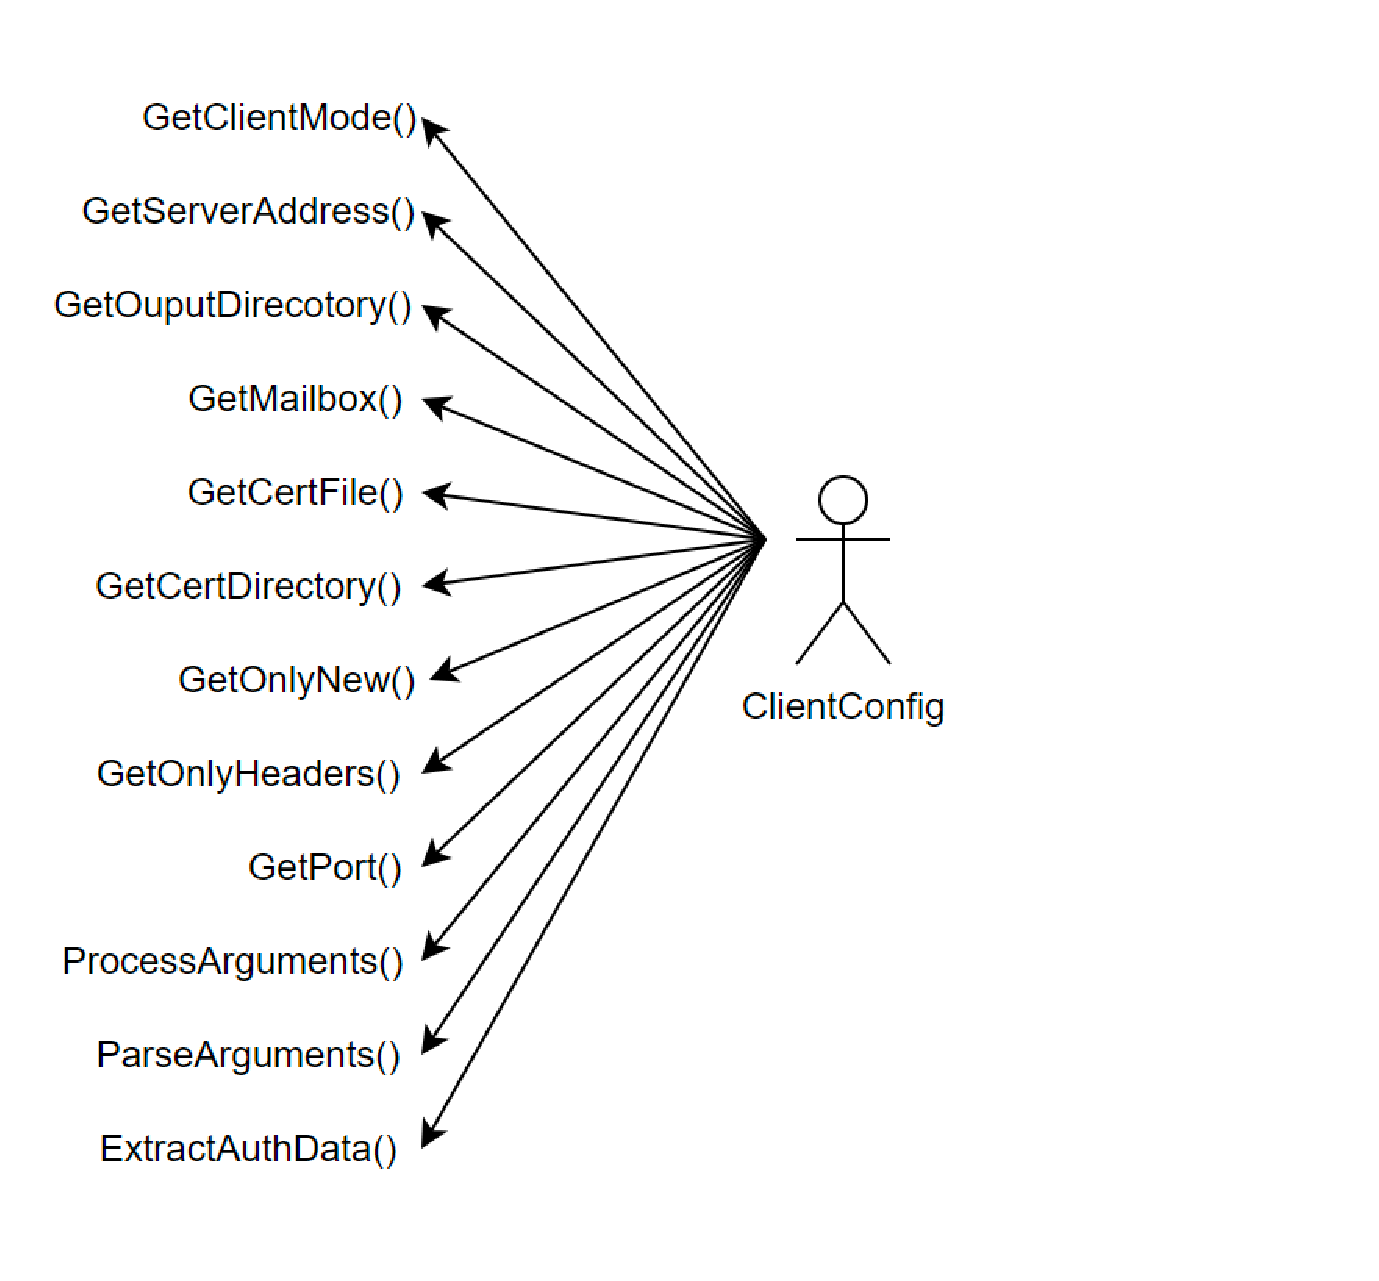
\includegraphics{ClientConfig.eps}
    }
    \caption{Program Flow Diagram}
    \label{figure:client-config}
\end{figure}

\begin{figure}[H]
    \centering
    \scalebox{0.4}{
        \includegraphics{ImapClient.eps}
    }
    \caption{Program Flow Diagram}
    \label{figure:imap-clients}
\end{figure}

\newpage

\section{Return Codes}
The program is designed in such a way that in case of an error or failure, the user 
is always informed about the situation that has occurred. In case of success the program 
always returns the return value 0 (respectively \verb!SUCCESS!), in other cases the program gives the return 
values according to the table below.

\begin{center}
    \vspace{0.5cm} % % Space before table
    \begin{tabularx}{\textwidth}{|>{\raggedright\arraybackslash}p{6.5cm}|>{\raggedright\arraybackslash}p{2cm}|>{\raggedright\arraybackslash}p{1.5cm}|>{\raggedright\arraybackslash}X|}
        \hline
        \textbf{Name} & \textbf{Data Type} & \textbf{Value} & \textbf{Description} \\
        \hline
        OUTPUT\_DIR\_NOT\_CREATED & int & -7 & Output Directory Could Not Be Created \\
        \hline
        UIDVALIDITY\_FILE\_NOT\_FOUND & int & -6 & .uidvalidity File Not Found \\
        \hline
        UIDVALIDITY\_FILE\_ERROR & int & -5 & Error With .uidvalidity File (Invalid Format, Out of Range) \\
        \hline
        CREATE\_CONNECTION\_FAILED & int & -4 & Failed to Create Connection With IMAP Server \\
        \hline
        SSL\_CERT\_VERIFICATION\_FAILED & int & -3 & SSL Certificate Verification Failed \\
        \hline
        FETCH\_EMAIL\_FAILED & int & -2 & Fetching Email By UID Failed \\
        \hline
        SUCCESS & int & 0 & Operation Was Successful \\
        \hline
        NO\_IP\_ADDR\_FOUND & int & 1 & No IPv4 Address Was Found \\
        \hline
        PARSE\_ARGUMENTS\_FAILED & int & 2 & Parsing Program's Arguments Failed \\
        \hline
        PARSE\_CREDENTIALS\_FAILED & int & 3 & Parsing Credentials Failed \\
        \hline
        SERVER\_UNKNOWN\_RESPONSE & int & 4 & Server Sent an Unknown Response \\
        \hline
        TRANSMIT\_DATA\_FAILED & int & 5 & Transmission of Data Failed \\
        \hline
        RECEIVE\_DATA\_FAILED & int & 6 & Reception of Data Failed \\
        \hline
        RESPONSE\_NOT\_FOUND & int & 7 & Expected Server's Response Was Not Found \\
        \hline
        PARSE\_BY\_REGEX\_FAILED & int & 8 & Parsing of Regular Expression Failed \\
        \hline
        NON\_UIDS\_RECEIVED & int & 9 & No UIDs Were Received From The IMAP Server \\
        \hline
        CONTINUE\_IN\_RECEIVING & int & 10 & Continue Receiving More Data \\
        \hline
        UNDEFINED\_STATE & int & 11 & Undefined State Encountered \\
        \hline
        UID\_VALIDITY\_ERROR\_IN\_RECV & int & 14 & Unable to Receive UIDVALIDITY From The Server \\
        \hline
        REMOVAL\_OF\_EMAILS\_FAILED & int & 15 & Failed to Remove Emails When UIDVALIDITY Does Not Match \\
        \hline
        BAD\_RESPONSE & string & "Bad Response :(" & Error During Receiving of Server's Response \\
        \hline
    \end{tabularx}
    \vspace{0.5cm} % Space after table
\end{center}


\bibliographystyle{unsrt}
\bibliography{resources}      
\end{document}
